%Every LaTeX file needs a documentclass declaration.
%Possibilities are article, book, letter.  Font size is also declared.

\documentclass[10pt]{article}

%special packages used for symbols, formatting, etc.

\usepackage{amsmath} % contains the align* environment, which is great for manipulating formulas
\usepackage{amssymb} % contains common symbols
\usepackage{amsthm} % has the proof environment
\usepackage[margin=1in]{geometry} % specifies page properties, such as the margin
%\usepackage{siunitx} % useful for typesetting units
\usepackage{tikz} % useful for graphics

% Define a lemma environment
% Set the style of the new theorem environments so that the text isn't in italics
\theoremstyle{definition}
% Define lemma environment, the first argument is the name in LaTeX, the second argument is what is typeset
\newtheorem{lemma}{Lemma}

% User-defined commands

\newcommand{\newprob}{\medskip \hrule \medskip}
\newcommand{\fanc}[1]{\mathbb{#1}}
\newcommand{\rn}[1]{\fanc{R}^{#1}}
\def\qed{\hspace*{\fill}\rule{1.854mm}{3mm}}  % the fancy box at the end of a proof

%%%%%%%%%%%%%%%%%%%%%%%%%%%%%%%%%%%%%%%%%%%%%%

%beginning of document, every \begin{} also requires an \end{} command.

%\renewcommand{\baselinestretch}{2}

\begin{document}

\pagestyle{empty}  %suppress page numbers, etc.

\begin{center}  %center command, also see flushright, flushleft

{\bf MATH 423-01  Advanced Calculus I

Homework \#8

Assigned: November 10, 2022

Due: November 17, 2022}

\end{center}

\medskip

\hrule   %horizontal line

\bigskip

% list environment: description, itemize, and enumerate

\begin{enumerate}

%%%%%%%%%%%%%%%%%%%%%%

\item  ~[Kline, L.] Prove that if $f$ is continuous on $[a,b]$ with $f(x) > 0$, for all $a \leq x \leq b$, then $1/f$ is bounded on $[a,b]$.  Hint: since continuity works with any $\varepsilon$, figure out what cleverly chosen $\varepsilon$ will be needed here, much like our usual Step 0.

%%%%%%%%
	
%\item  Decide on the validity of the following conjectures.  Provide either a counterexample or a proof.
%
%	\begin{enumerate}
%	
%	\item  Continuous functions take bounded open intervals to bounded open intervals.
%	
%	\item  Continuous functions take bounded open intervals to open sets.
%	
%	\item  Continuous functions take bounded closed intervals to bounded closed intervals.
%	
%	\end{enumerate}
	
%%%%%%%%%%%%%

\item  ~[Krason, T.] Let $f$ be a continuous function on the closed interval $[0,1]$, whose range is also contained in $[0,1]$.  Prove that $f$ must have a \emph{fixed point}. (Prove that $f(x) = x$, for at least one value of $x \in [0,1]$).  Hint: use our version of the Intermediate Value Theorem that concerns roots and a cleverly chosen function.
	
%%%%%%%%%%%%%%

\item  ~[Lauen, A.] Show that $f(x) = 1/x^2$ is uniformly continuous on the set $[1,\infty)$ but not on the set $(0,1]$.  Hint: use the examples from the notes for inspiration on bounding extra terms, and don't forget that we have a tool for showing that a function is not uniformly continuous. 
	
%%%%%%%%%%%%

\item  ~[Everyone, Lewis, J.] Assume that $f:[0,\infty) \to \mathbb{R}$ is continuous at every point in its domain.  Show that if there exists $b > 0$ such that $f$ is uniformly continuous on the set $[b,\infty)$, then $f$ is uniformly continuous on $[0,\infty)$.  Hint: note that $[0,b]$ is compact.

%%%%%%%%%%

\item  ~[Lindskov, I.] Construct an alternate proof of the theorem we proved in class that states

``A function that is continuous on a compact set $K$ is uniformly continuous on $K$.''

using the open cover definition of compactness.  Hint: let $\varepsilon > 0$.  For every point $p \in K$ we can choose $\delta_p > 0$ such that whenever $|x-p| < \delta_p$ it must be that $|f(x) - f(p)| < \frac{\varepsilon}{2}$.  Consider the open cover defined by $$J(p) = \left\{ x \in K: |x-p| < \frac{1}{2}\delta_p \right\}.$$  In this problem we need to cleverly choose not just $\varepsilon$ but also $\delta$.  The choice of $\delta$ I've suggested for the open cover is designed to help with that.
	
%%%%%%%%%%%%

\item  In class we used the Nested Interval Property to prove the Intermediate Value Theorem (IVT).  This is another statement that can be used to prove all of the other statements we have proven so far.  This updates Figure \ref{fig:theorems}.

	\begin{figure}[h]
	\begin{center}
	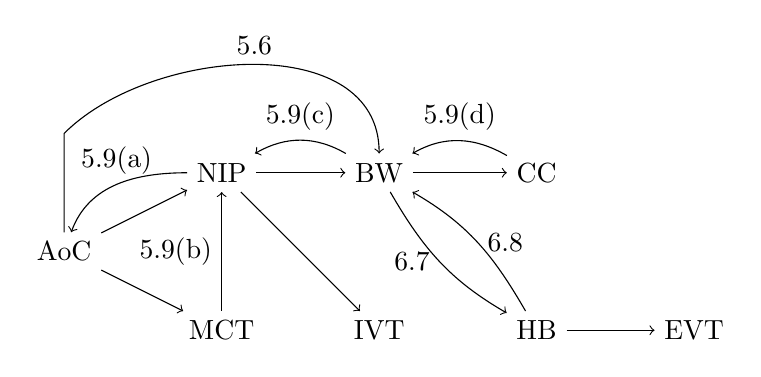
\begin{tikzpicture}
	
	% Draw nodes
	\node (AoC) at (0,0) {AoC};
	\node (MCT) at (2,-1) {MCT};
	\node (NIP) at (2,1) {NIP};
	\node (BW) at (4,1) {BW};
	\node (CC) at (6,1) {CC};
	\node (HB) at (6,-1) {HB};
	\node (EVT) at (8,-1) {EVT};
	\node (IVT) at (4,-1) {IVT};
	
	% Draw arcs, what we have proved in class or the homework
	\draw[->] (AoC) to (MCT);
	\draw[->] (AoC) to (NIP);
	\draw[->] (NIP) to (BW);
	\draw[->,in=90] (AoC) |- (0,1.5) to node[midway,above] {5.6} (BW);
	\draw[->] (BW) to (CC);
	\draw[->,out=180,in=70] (NIP) to node[midway,above] {5.9(a)} (AoC);
	\draw[->] (MCT) to node[midway,left] {5.9(b)} (NIP);
	\draw[->,out=150,in=30] (BW) to node[midway,above] {5.9(c)} (NIP);
	\draw[->,out=150,in=30] (CC) to node[midway,above] {5.9(d)} (BW);
	\draw[->,out=-60,in=150] (BW) to node[midway,left] {6.7} (HB);
	\draw[->,out=120,in=-30] (HB) to node[midway,right] {6.8}  (BW);
	
	% Draw arcs, what we will prove here
	\draw[->] (HB) to (EVT);
	\draw[->] (NIP) to (IVT);
	
	\end{tikzpicture}
	\caption{A directed graph showing the logical implications of the various statements.}\label{fig:theorems}
	\end{center}
	\end{figure}
	
	%%%%%%%%%
	
	As before, if you can add an arrow to this graph, it is worth extra credit.
	
%%%%%%%%%%%%%

\end{enumerate}

\end{document}
